\section{问题一：单点往返运输能力与货箱组批}
\label{sec:q1}

\subsection{问题分析与模型建立}

问题一不含实体无人机与电池调度，因此可拆为两个层次：\textbf{载荷层}——确定每种机型在每个服务区的最大安全载荷；\textbf{组批层}——把该服务区的货箱装入最少的架次。每个架次的形式固定为 $O01\to S_i\to O01$，仅服务一个服务区、不得跨服务区组批；同一服务区可由多个架次分批服务。

\textbf{（1）载荷层。}对每个 $(g,i)$ 组合，按式~\eqref{eq:8} 反解能量约束取等号时的载荷 $q_{max}^{energy}$，再与结构上限 $Q_{g}$ 和体积瓶颈对应质量取小，得到 $q_{max}^{safe}(g,i)$。

\textbf{（2）组批层。}设服务区 $S_i$ 的货箱集合为 $\mathcal{B}_i$，需将其划分为最少的子集（架次）$\{p_1,p_2,\dots\}$，使每个架次同时满足\textbf{质量约束}与\textbf{体积约束}：
\begin{equation}
	\label{eq:19}
	\sum_{b\in p}m_{b}\le q_{max}^{safe}(g,i),\qquad \sum_{b\in p}v_{b}\le V_{g}
\end{equation}
这是一个\textbf{质量—体积二维装箱问题}\cite{martello1990binpacking,lodi2002threedim}，且机型 $g$ 本身也是决策变量。由于同一类物资的单箱质量与体积取值唯一（见图~\ref{fig:boxes}(c)），问题实例具有良好的结构，适合用 FFD（First-Fit Decreasing）构造并用解析下界验证最优性。

\textbf{（3）解析下界。}构造 Martello--Toth 型下界\cite{martello1990binpacking}：分别按\textbf{质量}与\textbf{体积}两个维度，用该服务区可获得的最佳机型容量估计所需架次数，取二者较大值：
\begin{equation}
	\label{eq:20}
	LB_i=\max\left(\left\lceil\frac{\sum_{b\in\mathcal{B}_i}m_{b}}{\max_{g}q_{max}^{safe}(g,i)}\right\rceil,\
	\left\lceil\frac{\sum_{b\in\mathcal{B}_i}v_{b}}{\max_{g}V_{g}}\right\rceil\right)
\end{equation}
若启发式解的架次数等于 $LB_i$，则在该服务区上\textbf{架次数维度可证最优}。

\subsection{求解算法}

求解流程如图~\ref{fig:flow_q1} 所示。

\begin{figure}[htbp]
	\centering
	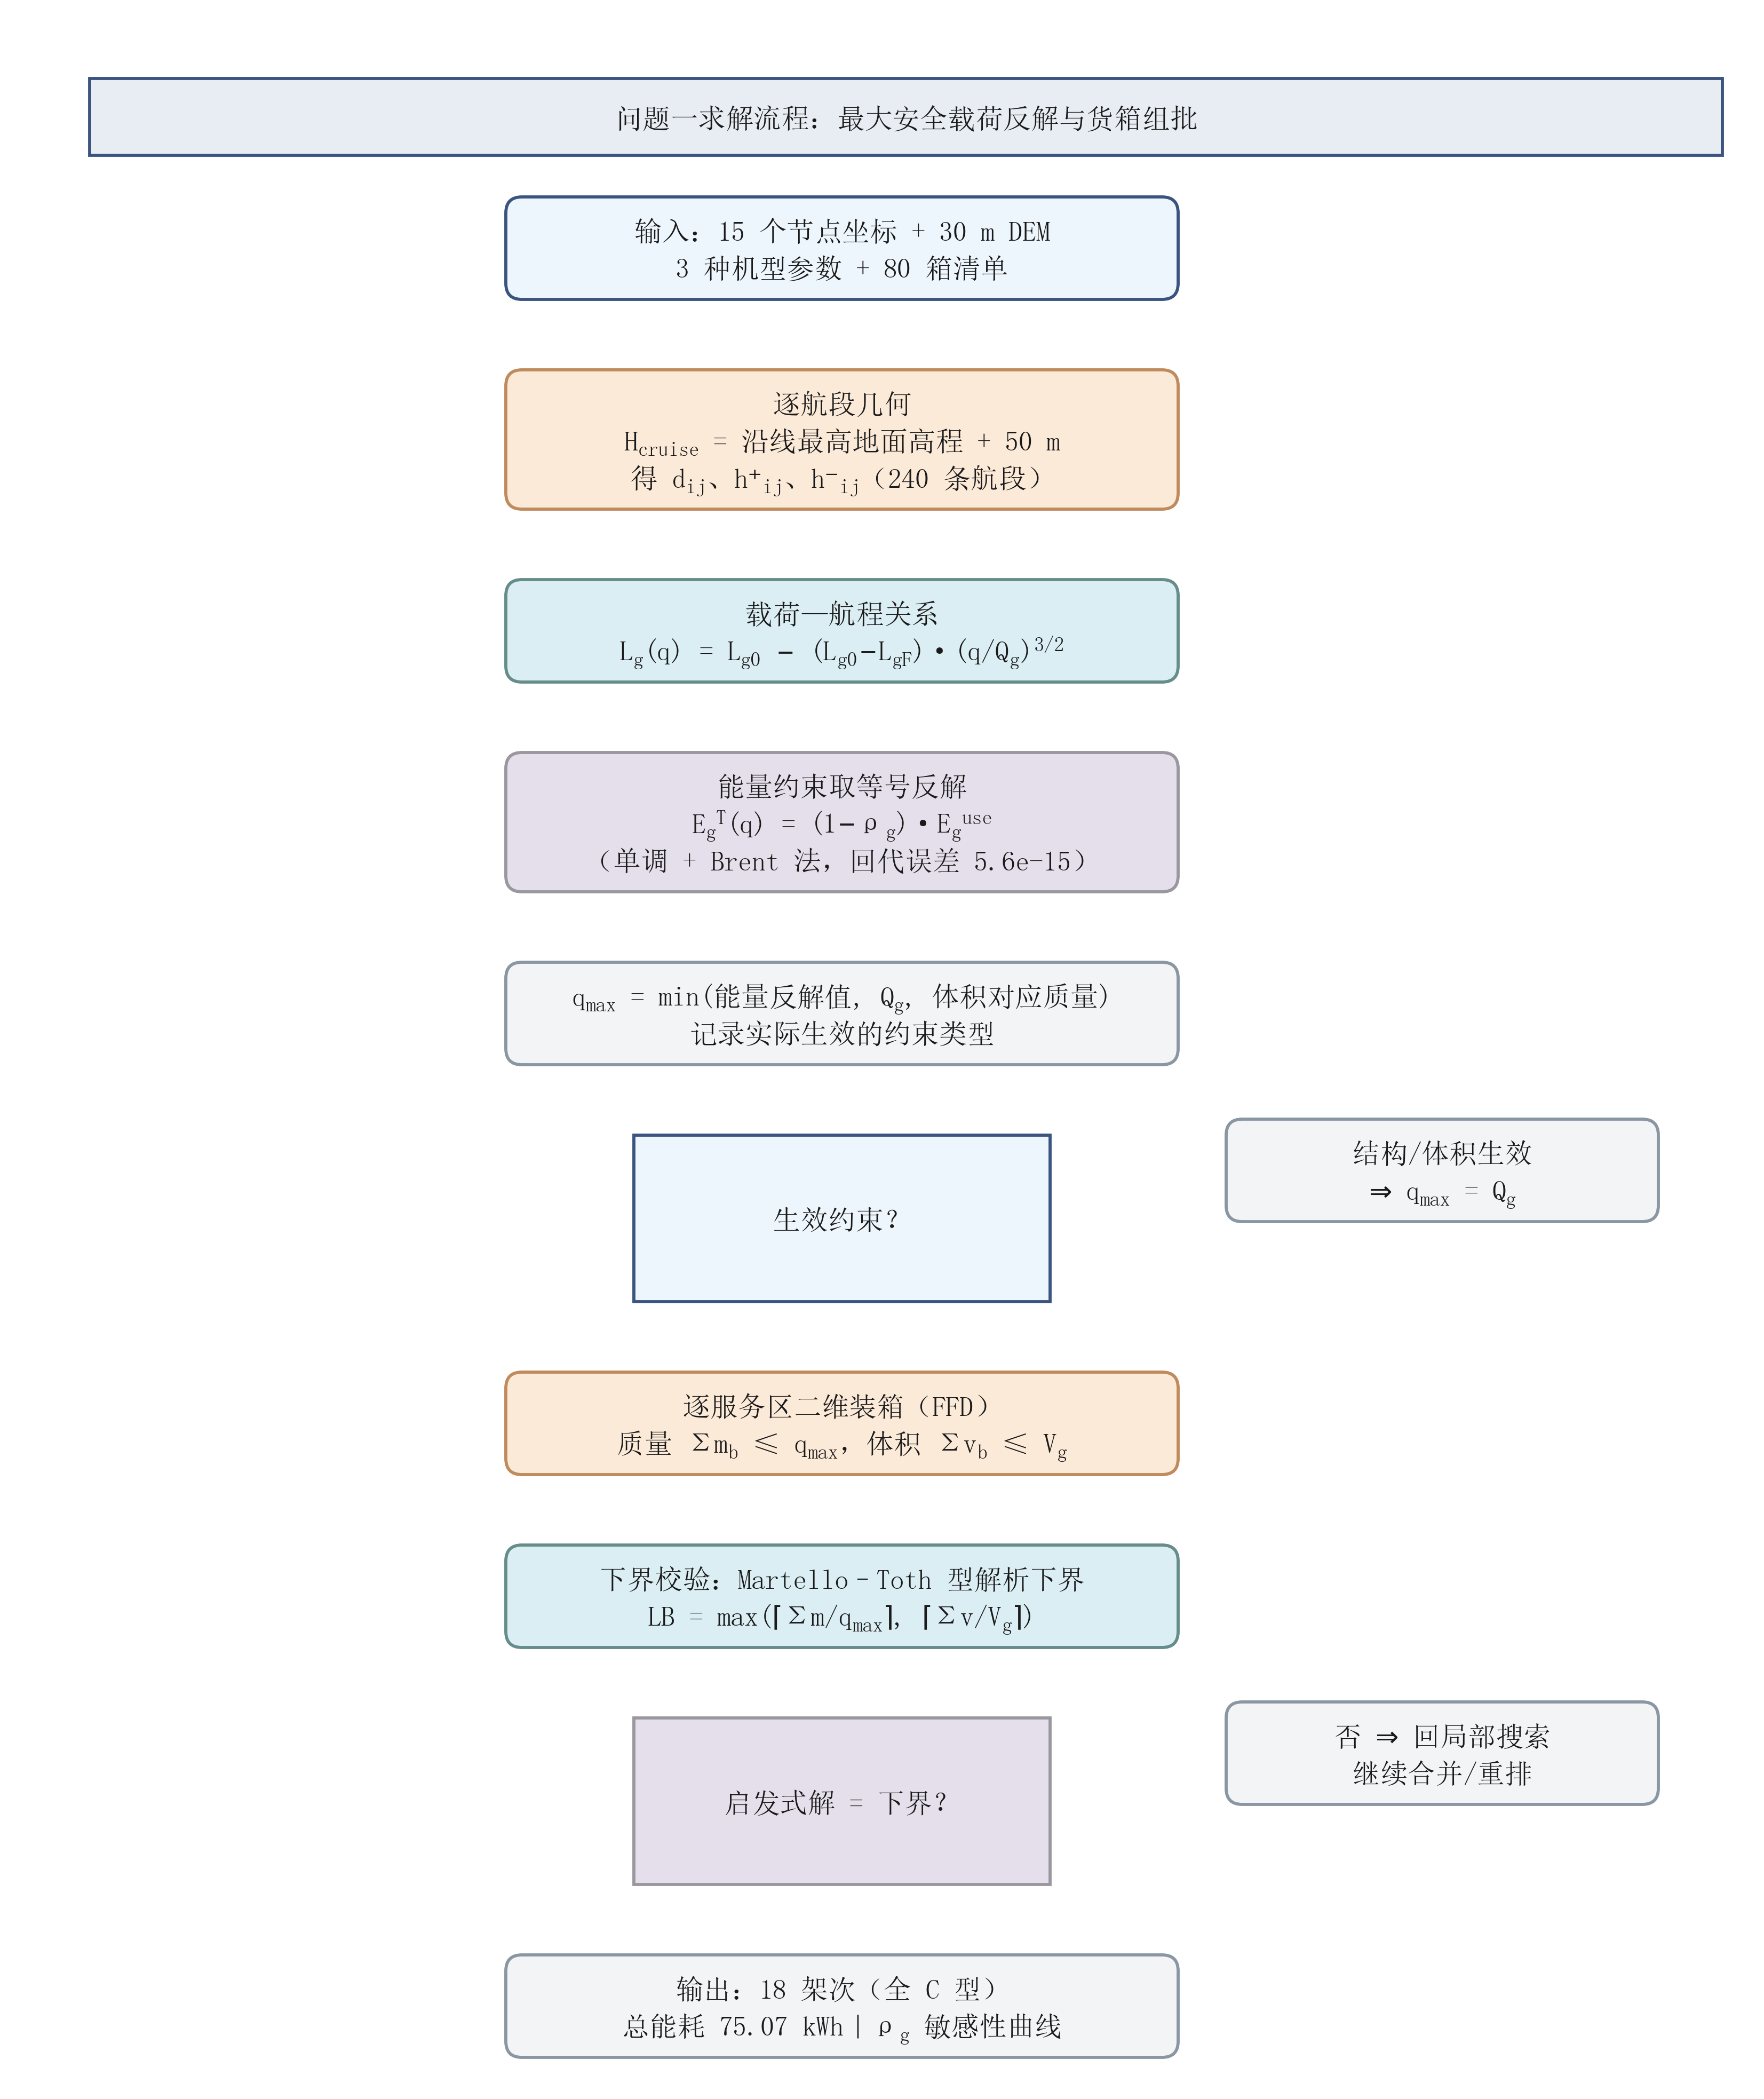
\includegraphics[width=0.86\textwidth]{figures/fig02_flow_q1.png}
	\caption{问题一求解流程}
	\label{fig:flow_q1}
\end{figure}

算法分五步（见图~\ref{fig:flow_q1}）：\textbf{①}由 DEM 沿航段采样最高地面高程，得到 240 条航段的 $d_{ij}$、$h^{+}_{ij}$、$h^{-}_{ij}$；\textbf{②}按式~\eqref{eq:4} 建立载荷—航程关系；\textbf{③}用单调性 $+$ Brent 法反解能量约束，得到 $q_{max}^{energy}$，并与 $Q_{g}$、体积上限取小，同时\textbf{记录实际生效的约束类型}；\textbf{④}对每个服务区独立做 FFD 二维装箱；\textbf{⑤}用式~\eqref{eq:20} 的解析下界校验最优性，若存在差距则回局部搜索继续合并重排。

\subsection{计算结果}

\subsubsection{最大安全载荷与生效约束}

3 种机型 $\times$ 15 个服务区的最大安全载荷及其生效约束如图~\ref{fig:q1_payload} 与表~\ref{tab:q1_payload} 所示。

\begin{table}[htbp]
\caption{3 机型 $\times$ 15 服务区最大安全载荷与生效约束}
\label{tab:q1_payload}
\centering
\zihao{-5}
\setlength{\tabcolsep}{4pt}
\begin{tabular}{lcccc}
\toprule
服务区 & 单向距离 / km & A 型载荷 / kg & B 型载荷 / kg & C 型载荷 / kg \\
\midrule
S001 & 3.05 & 25.0（结构） & 30.0（结构） & 80.0（结构） \\
S002 & 7.41 & 25.0（结构） & 30.0（结构） & 68.9（能量） \\
S003 & 7.26 & 25.0（结构） & 30.0（结构） & 68.3（能量） \\
S004 & 7.71 & 25.0（结构） & 30.0（结构） & 63.7（能量） \\
S005 & 5.28 & 25.0（结构） & 30.0（结构） & 80.0（结构） \\
S006 & 3.19 & 25.0（结构） & 30.0（结构） & 80.0（结构） \\
S007 & 4.53 & 25.0（结构） & 30.0（结构） & 80.0（结构） \\
S008 & 8.08 & 25.0（结构） & 28.9（能量） & 59.0（能量） \\
S009 & 5.71 & 25.0（结构） & 30.0（结构） & 80.0（结构） \\
S010 & 4.78 & 25.0（结构） & 30.0（结构） & 80.0（结构） \\
S011 & 2.81 & 25.0（结构） & 30.0（结构） & 80.0（结构） \\
S012 & 7.39 & 25.0（结构） & 30.0（结构） & 68.1（能量） \\
S013 & 4.85 & 25.0（结构） & 30.0（结构） & 80.0（结构） \\
S014 & 5.42 & 25.0（结构） & 30.0（结构） & 80.0（结构） \\
S015 & 6.01 & 25.0（结构） & 30.0（结构） & 80.0（结构） \\
\bottomrule
\end{tabular}
\\[2pt] \footnotesize 注：括号内为该组合实际生效的约束类型。
\end{table}


\begin{figure}[htbp]
	\centering
	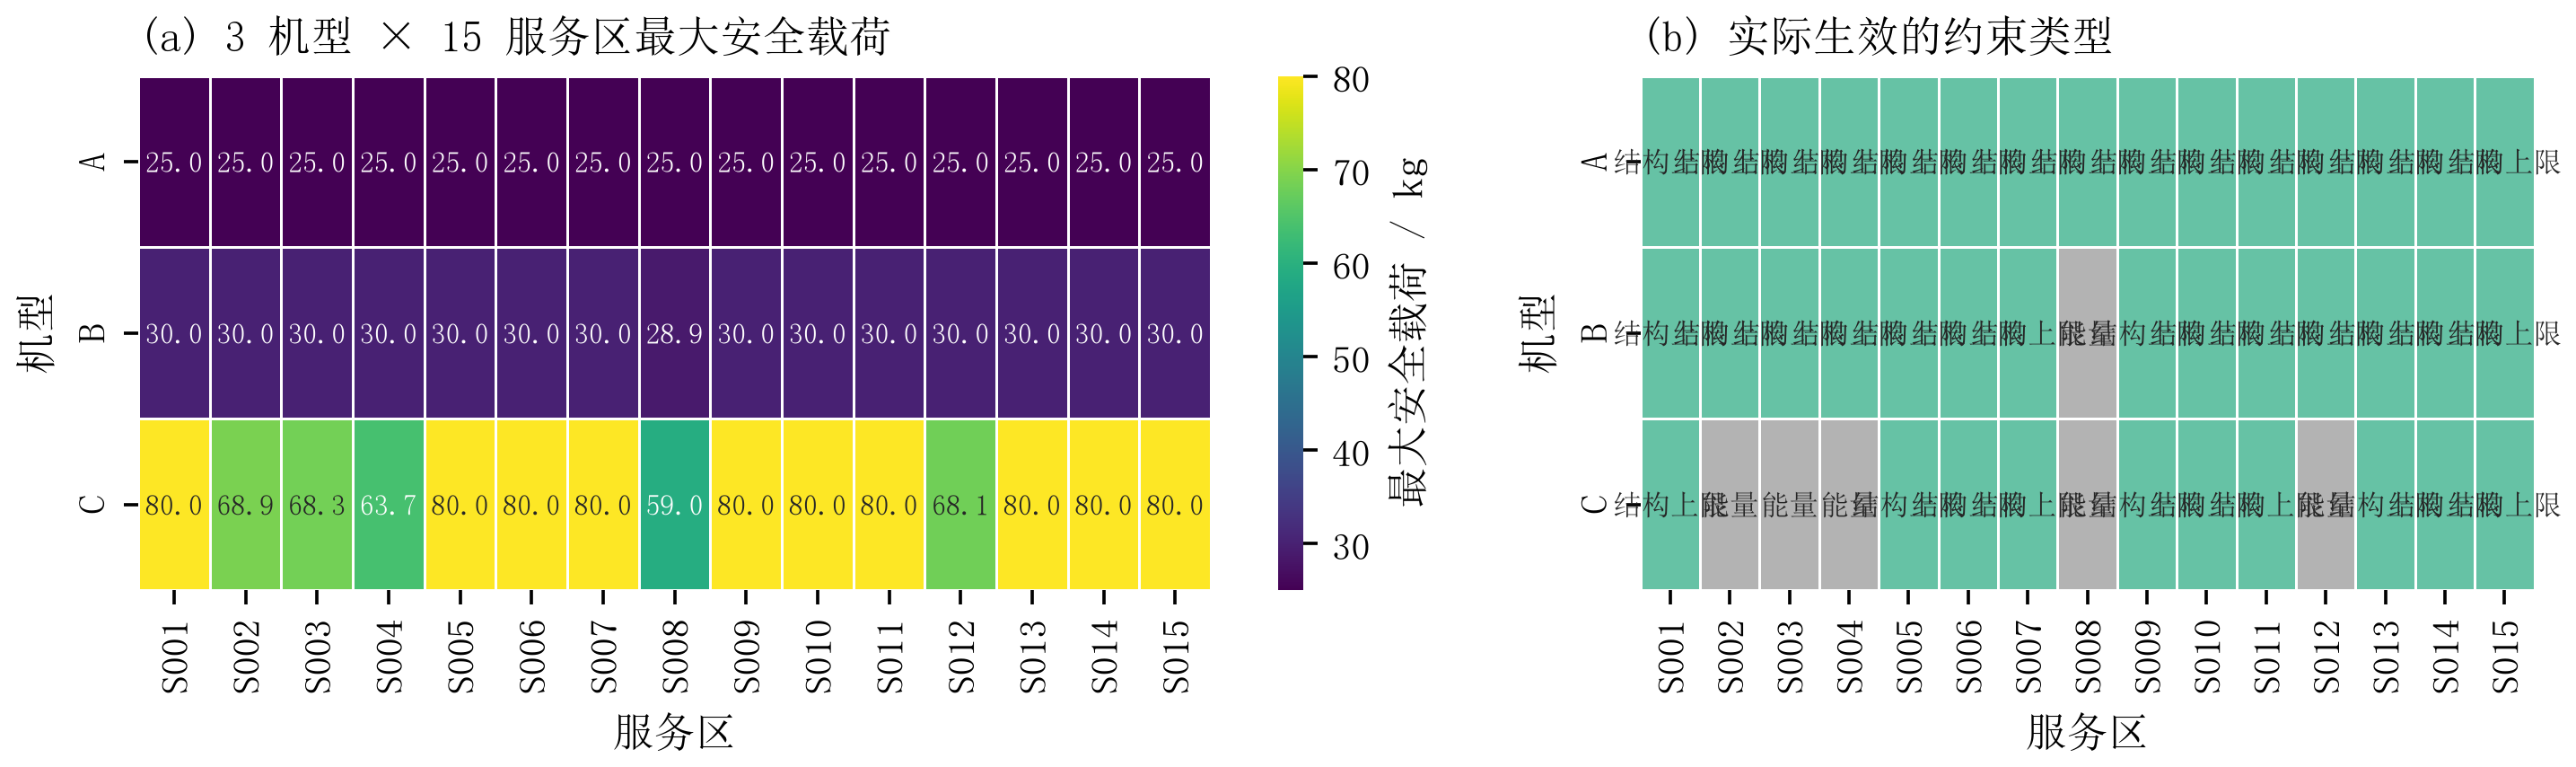
\includegraphics[width=0.98\textwidth]{figures/fig13_q1_payload_heatmap.png}
	\caption{最大安全载荷热力图与生效约束}
	\label{fig:q1_payload}
\end{figure}

一个\textbf{反直觉但十分关键}的结论是：\textbf{结构载重而非能量才是主导约束}。由图~\ref{fig:q1_binding}(a) 可见，\textbf{A 型在 15/15 个服务区全部受结构上限 $Q_{g}=25$\,kg 约束}，能量从未成为紧约束；B 型在 14/15 个服务区受结构约束（仅 S008 受能量约束，反解得 28.851\,kg）；只有 C 型因"重载且满载航程衰减最大"（53.8\%，见图~\ref{fig:uav_radar}(b)）而在 5 个远距离服务区触发电量约束。

\begin{figure}[htbp]
	\centering
	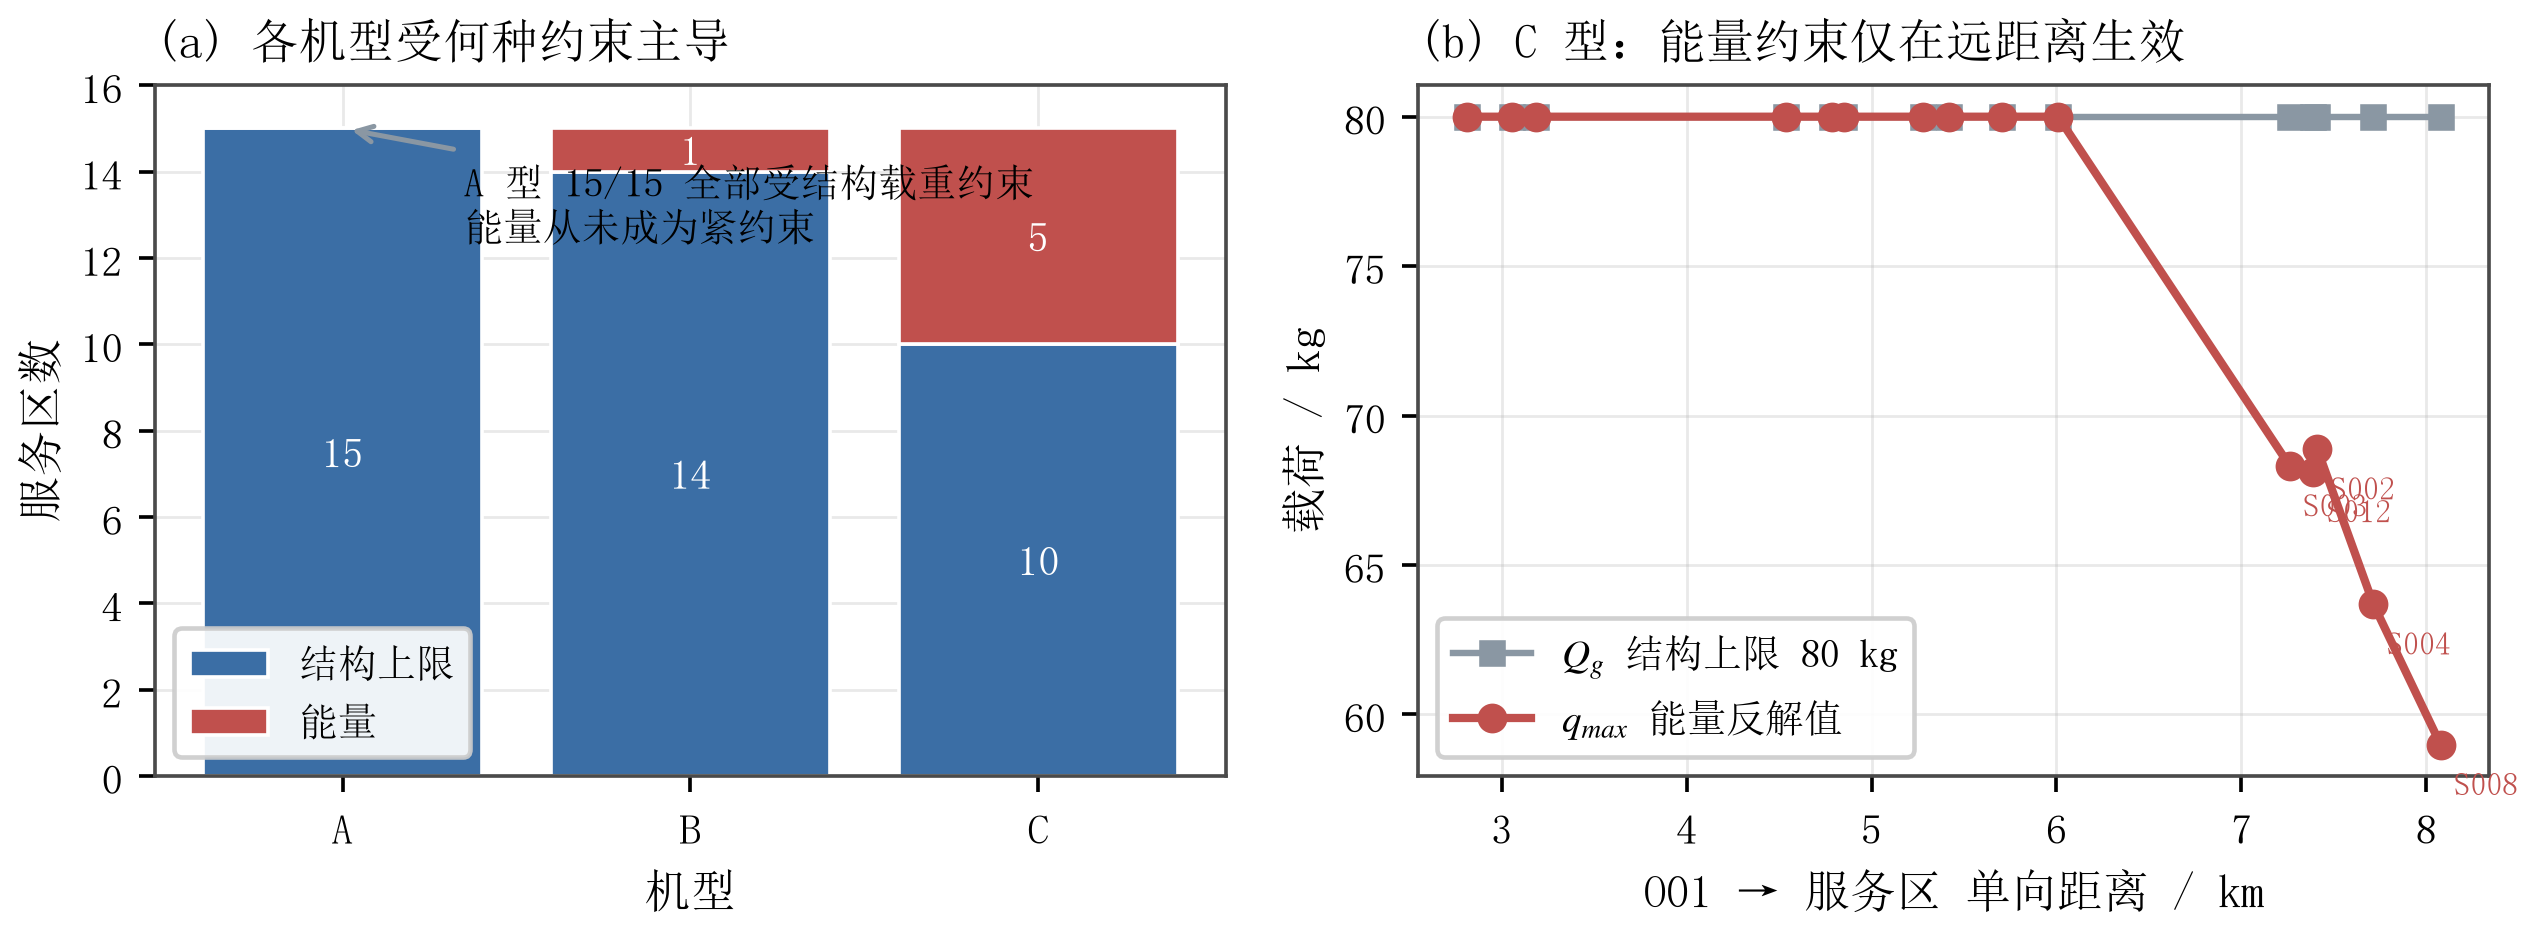
\includegraphics[width=0.98\textwidth]{figures/fig14_q1_binding.png}
	\caption{各机型生效约束与 C 型的能量约束边界}
	\label{fig:q1_binding}
\end{figure}

图~\ref{fig:q1_binding}(b) 进一步揭示能量约束的触发规律：C 型的能量反解值随距离单调下降，在 7.3\,km 以外开始低于结构上限 80\,kg。具体地，S002（7.41\,km）反解得 68.884\,kg、S012（7.39\,km）68.121\,kg、S003（7.26\,km）68.317\,kg、S004（7.71\,km）63.695\,kg，最远的 S008（8.08\,km）仅 58.990\,kg。这条"距离—载荷边界"是问题一中唯一需要真正数值反解的情形，也是后文 $\rho_{g}$ 敏感性的重点。

\subsubsection{货箱组批方案与最优性}

按上述算法得到\textbf{18 个架次、全部为 C 型}的组批方案，其构成如图~\ref{fig:q1_groups} 所示。

\begin{figure}[htbp]
	\centering
	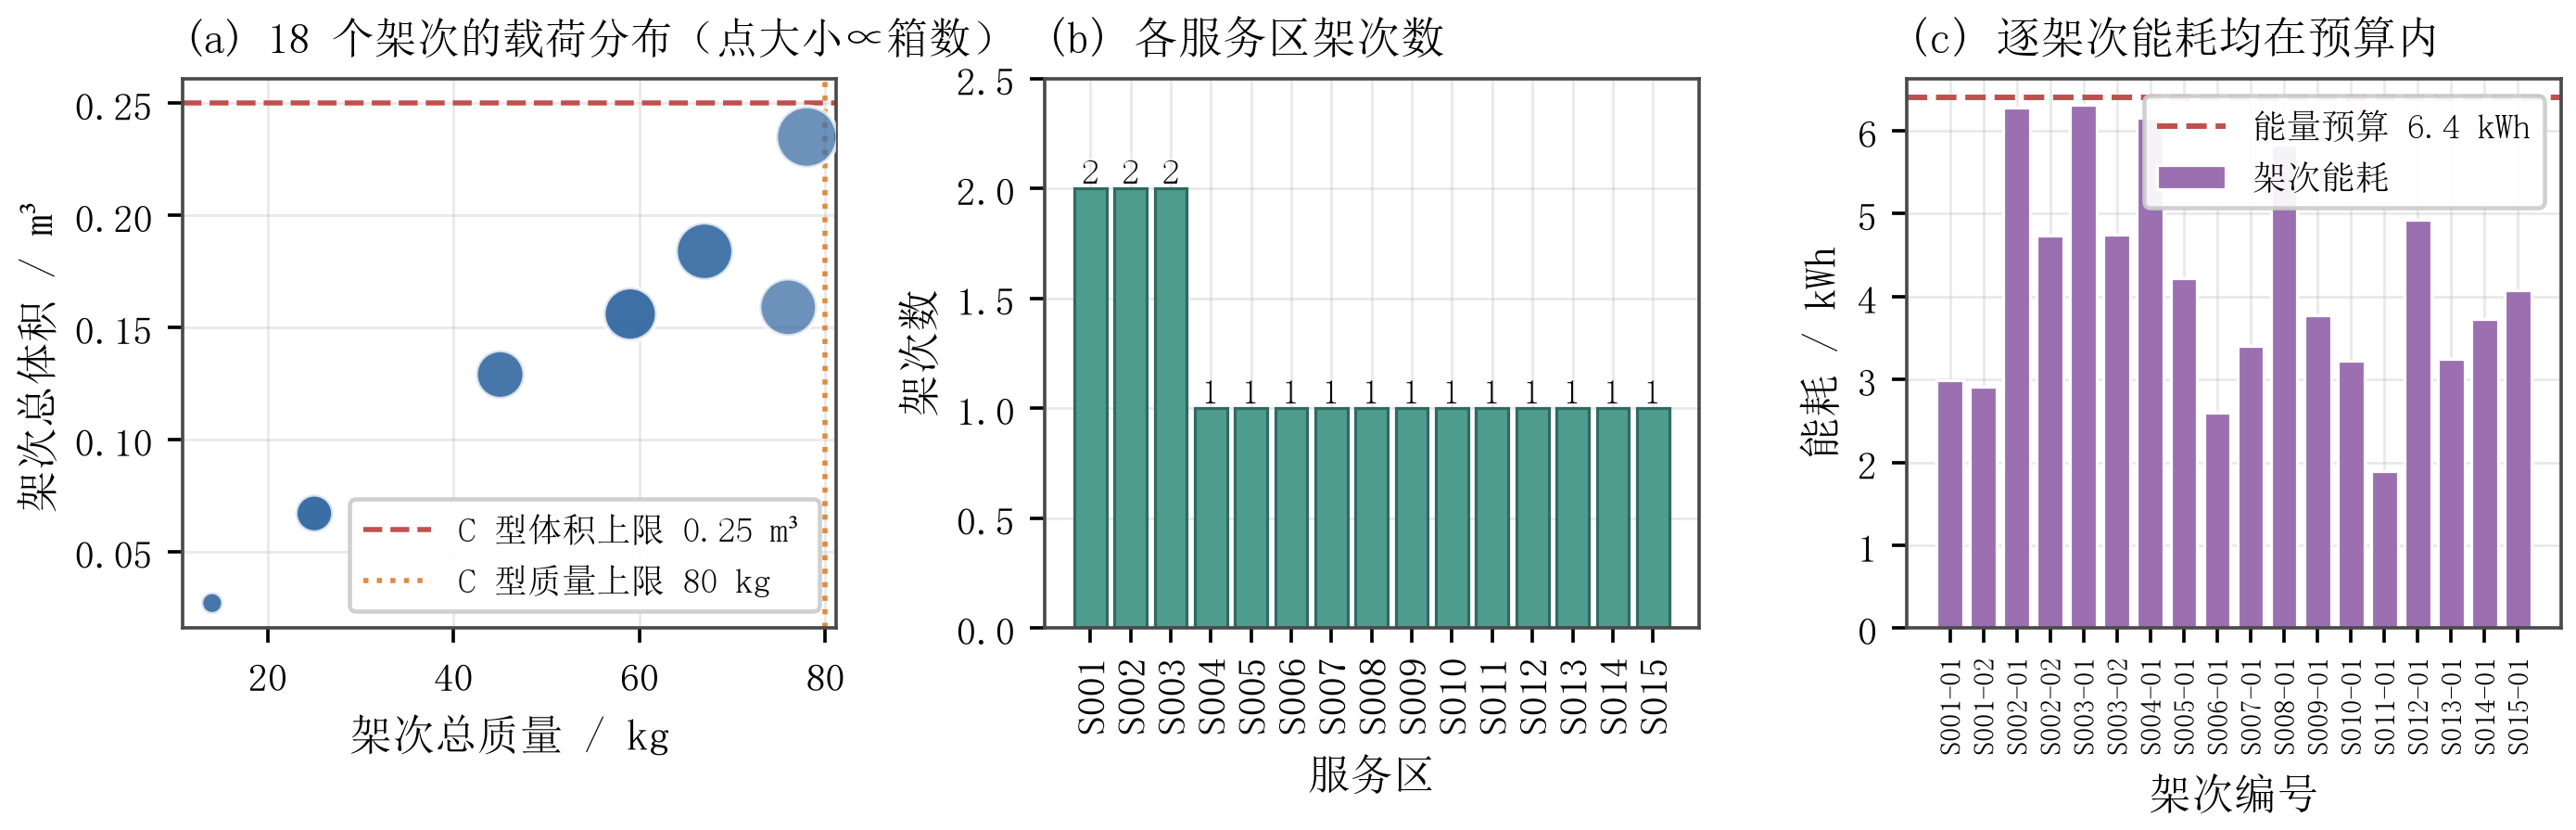
\includegraphics[width=0.98\textwidth]{figures/fig15_q1_groups.png}
	\caption{货箱组批方案构成}
	\label{fig:q1_groups}
\end{figure}

由图~\ref{fig:q1_groups}(a) 可见，各架次的装载点密集分布在体积上限 0.25\,m$^3$ 附近而非质量上限 80\,kg 附近，这说明\textbf{体积比质量更紧}——例如 S001 的第一个架次装载 8 箱共 78.0\,kg、0.235\,m$^3$，质量尚有 2\,kg 余量而体积已接近上限。图~\ref{fig:q1_groups}(c) 验证了全部 18 个架次的能耗均在能量预算 6.4\,kWh 之内。

需要特别说明的是\textbf{A 型与 B 型几乎派不上用场}：其可用装载体积仅 0.06 / 0.073\,m$^3$，而任何服务区的总货量体积都 $\ge0.067$\,m$^3$（最小的 3 箱服务区即需 0.067\,m$^3$），因此 A/B 型只能用于拆分后的零散小批量，主力必然是 C 型。这也解释了为何最优方案中 18 个架次全部为 C 型。

\textbf{最优性验证。}图~\ref{fig:q1_lowerbound}(a) 给出了逐服务区的解析下界与启发式结果对比：\textbf{15 个服务区的架次数全部等于其解析下界}（S001、S002、S003 各需 2 个架次，其余 12 个各需 1 个，合计恰好 18），因此本文方案在\textbf{架次数维度上可证最优}。

\begin{figure}[htbp]
	\centering
	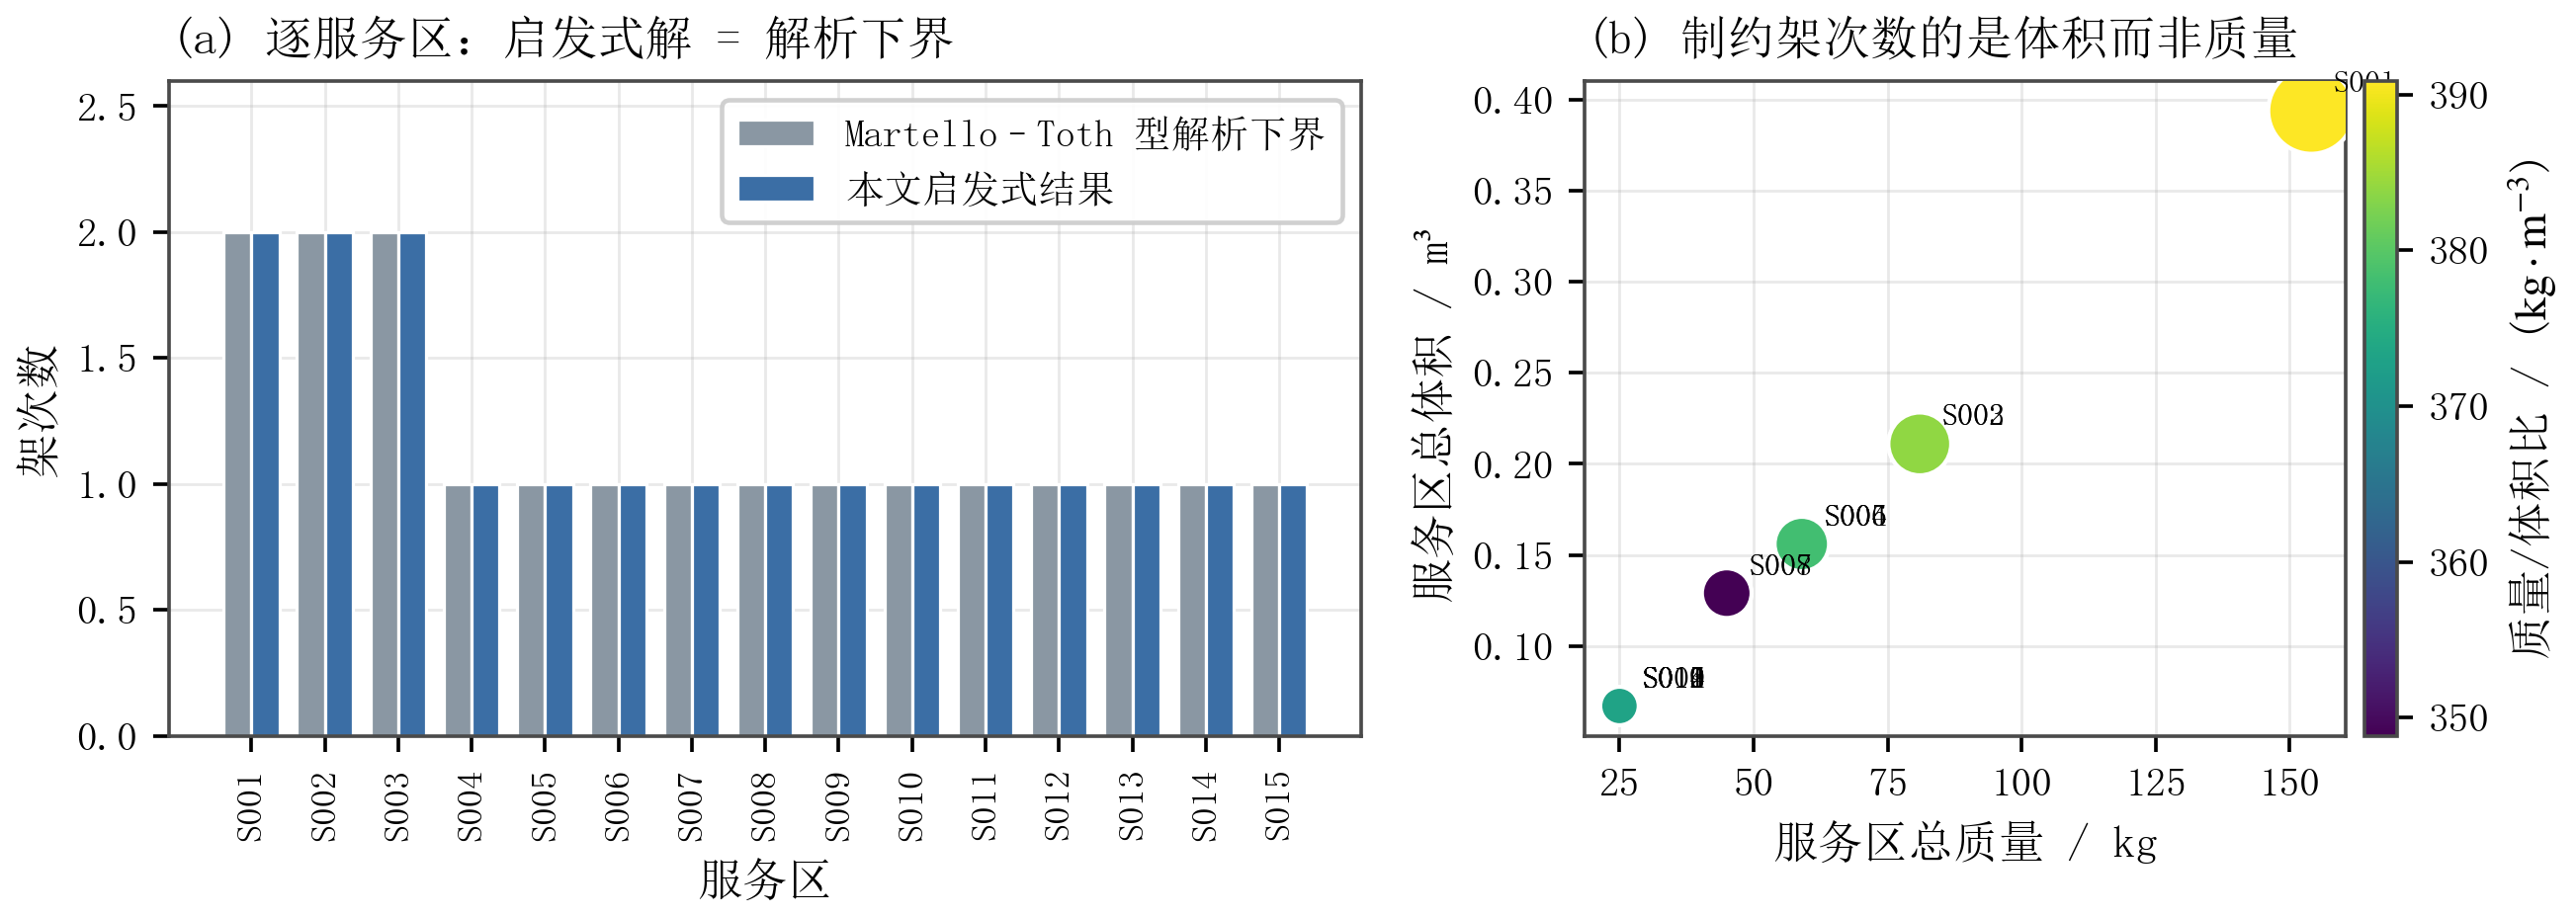
\includegraphics[width=0.98\textwidth]{figures/fig17_q1_lowerbound.png}
	\caption{逐服务区架次数下界与启发式差距}
	\label{fig:q1_lowerbound}
\end{figure}

图~\ref{fig:q1_lowerbound}(b) 揭示了制约架次数的根本原因是\textbf{体积而非质量}：各服务区的质量/体积比介于 300$\sim$400\,kg/m$^3$，普遍高于 C 型的装载密度上限（80\,kg / 0.25\,m$^3$ = 320\,kg/m$^3$），因此体积维度更容易先被填满。

\subsubsection{三目标权衡与策略对比}

本文对比了 8 种组批策略，其多目标表现如表~\ref{tab:q1_strategy} 与图~\ref{fig:q1_strategy} 所示。

\begin{table}[htbp]
\caption{各组批策略的多目标对比}
\label{tab:q1_strategy}
\centering
\zihao{-5}
\setlength{\tabcolsep}{4pt}
\begin{tabular}{llcccc}
\toprule
策略 & 说明 & 架次数 & 总能耗 / kWh & 累计作业 / h & 并行完工 / h \\
\midrule
ffd\_volume & FFD 体积降序 + 最大机型优 & 18 & 75.07 & 9.37 & 1.27 \\
single\_C & 全程只使用 C 型 & 18 & 75.07 & 9.37 & 1.27 \\
nf\_as\_given & 不排序（按附件顺序）+ 最大机型 & 18 & 75.07 & 9.37 & 1.27 \\
ffd\_mass & FFD 质量降序 + 最大机型优 & 18 & 75.07 & 9.37 & 1.27 \\
mixed\_largest\_first & 混合机型，新箱优先选最大机型 & 18 & 75.07 & 9.37 & 1.27 \\
single\_B & 全程只使用 B 型 & 37 & 72.86 & 16.31 & 2.25 \\
single\_A & 全程只使用 A 型 & 55 & 118.80 & 26.17 & 3.70 \\
mixed\_best\_fit & 混合机型，新箱优先选能装下的最小 & 55 & 118.80 & 26.17 & 3.70 \\
\bottomrule
\end{tabular}
\end{table}


\begin{figure}[htbp]
	\centering
	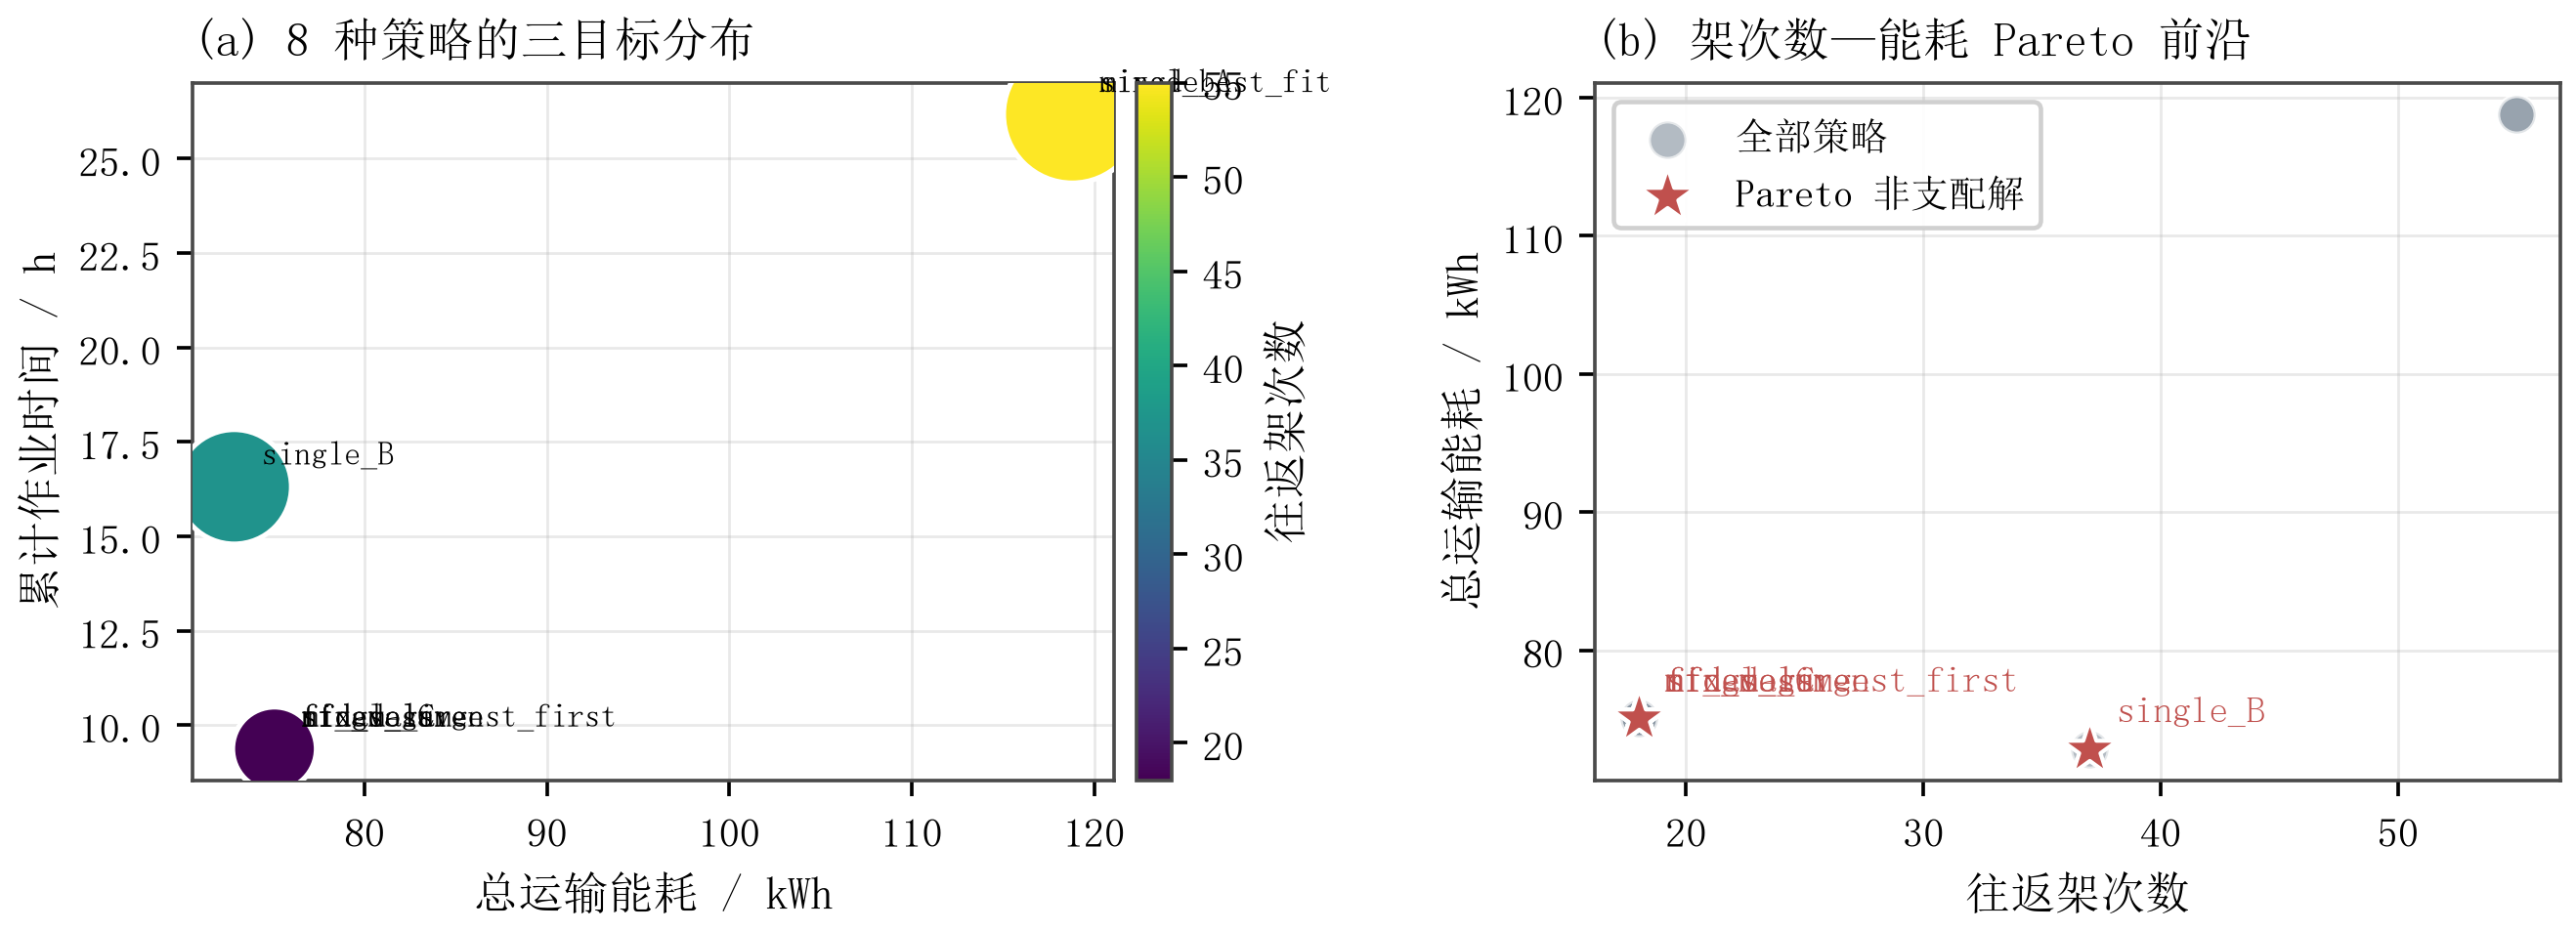
\includegraphics[width=0.98\textwidth]{figures/fig16_q1_strategy.png}
	\caption{策略对比与 Pareto 前沿}
	\label{fig:q1_strategy}
\end{figure}

由图~\ref{fig:q1_strategy}(b) 可见，8 种策略在"往返架次数—总运输能耗"平面上形成清晰的分层：5 种以 C 型为主的策略重合于 (18, 75.07)，单独使用 A 型的两种策略劣化至 (55, 118.80)，而\textbf{单独使用 B 型的策略落在 Pareto 前沿的另一端}——它以 \textbf{37 个架次}换取了 \textbf{72.86\,kWh} 的更低能耗。

这一权衡关系具有明确的工程含义：B 型的空载标准航程（28\,km）优于 C 型（26\,km），且机身更轻（65\,kg vs 69.9\,kg），因此\textbf{单位运输能耗更低}；但其载重与体积仅为 C 型的 37.5\% 与 29.2\%，导致需要近两倍的架次数、1.74 倍的累计作业时间与 1.77 倍的并行完工时间。因此在\textbf{应急场景下应以架次数与作业时间优先}，选择 18 架次的全 C 型方案；若场景转为对能耗敏感的长周期运输，则 B 型方案更优。

\subsubsection{返航安全余量敏感性分析}

返航安全余量 $\rho_{g}$ 直接决定了可用于飞行的能量上限 $(1-\rho_{g})E_{g}^{use}$，是最重要的安全参数。本文以 0.025 为步长在 $[0,0.50]$ 上扫描，逐点重算最大安全载荷并重跑组批，结果如图~\ref{fig:q1_rho}、图~\ref{fig:q1_rho_heatmap} 与表~\ref{tab:q1_rho_sweep} 所示。

\begin{table}[htbp]
\caption{返航安全余量 $\rho_{g}$ 扫描结果（节选）}
\label{tab:q1_rho_sweep}
\centering
\zihao{-5}
\setlength{\tabcolsep}{4pt}
\begin{tabular}{cccccc}
\toprule
$\rho_{g}$ & 架次数 & 总能耗 / kWh & 累计作业 / h & 有可行解 & 不可行服务区数 \\
\midrule
0.000 & 18 & 76.08 & 9.37 & 是 & 0 \\
0.100 & 18 & 76.08 & 9.37 & 是 & 0 \\
0.200 & 18 & 75.07 & 9.37 & 是 & 0 \\
0.225 & 18 & 74.79 & 9.37 & 是 & 0 \\
0.250 & 19 & 78.56 & 9.90 & 是 & 0 \\
0.275 & 20 & 83.47 & 10.42 & 是 & 0 \\
0.350 & 25 & 106.60 & 13.01 & 是 & 0 \\
0.375 & 0 & 0.00 & — & 否 & 1 \\
\bottomrule
\end{tabular}
\end{table}


\begin{figure}[htbp]
	\centering
	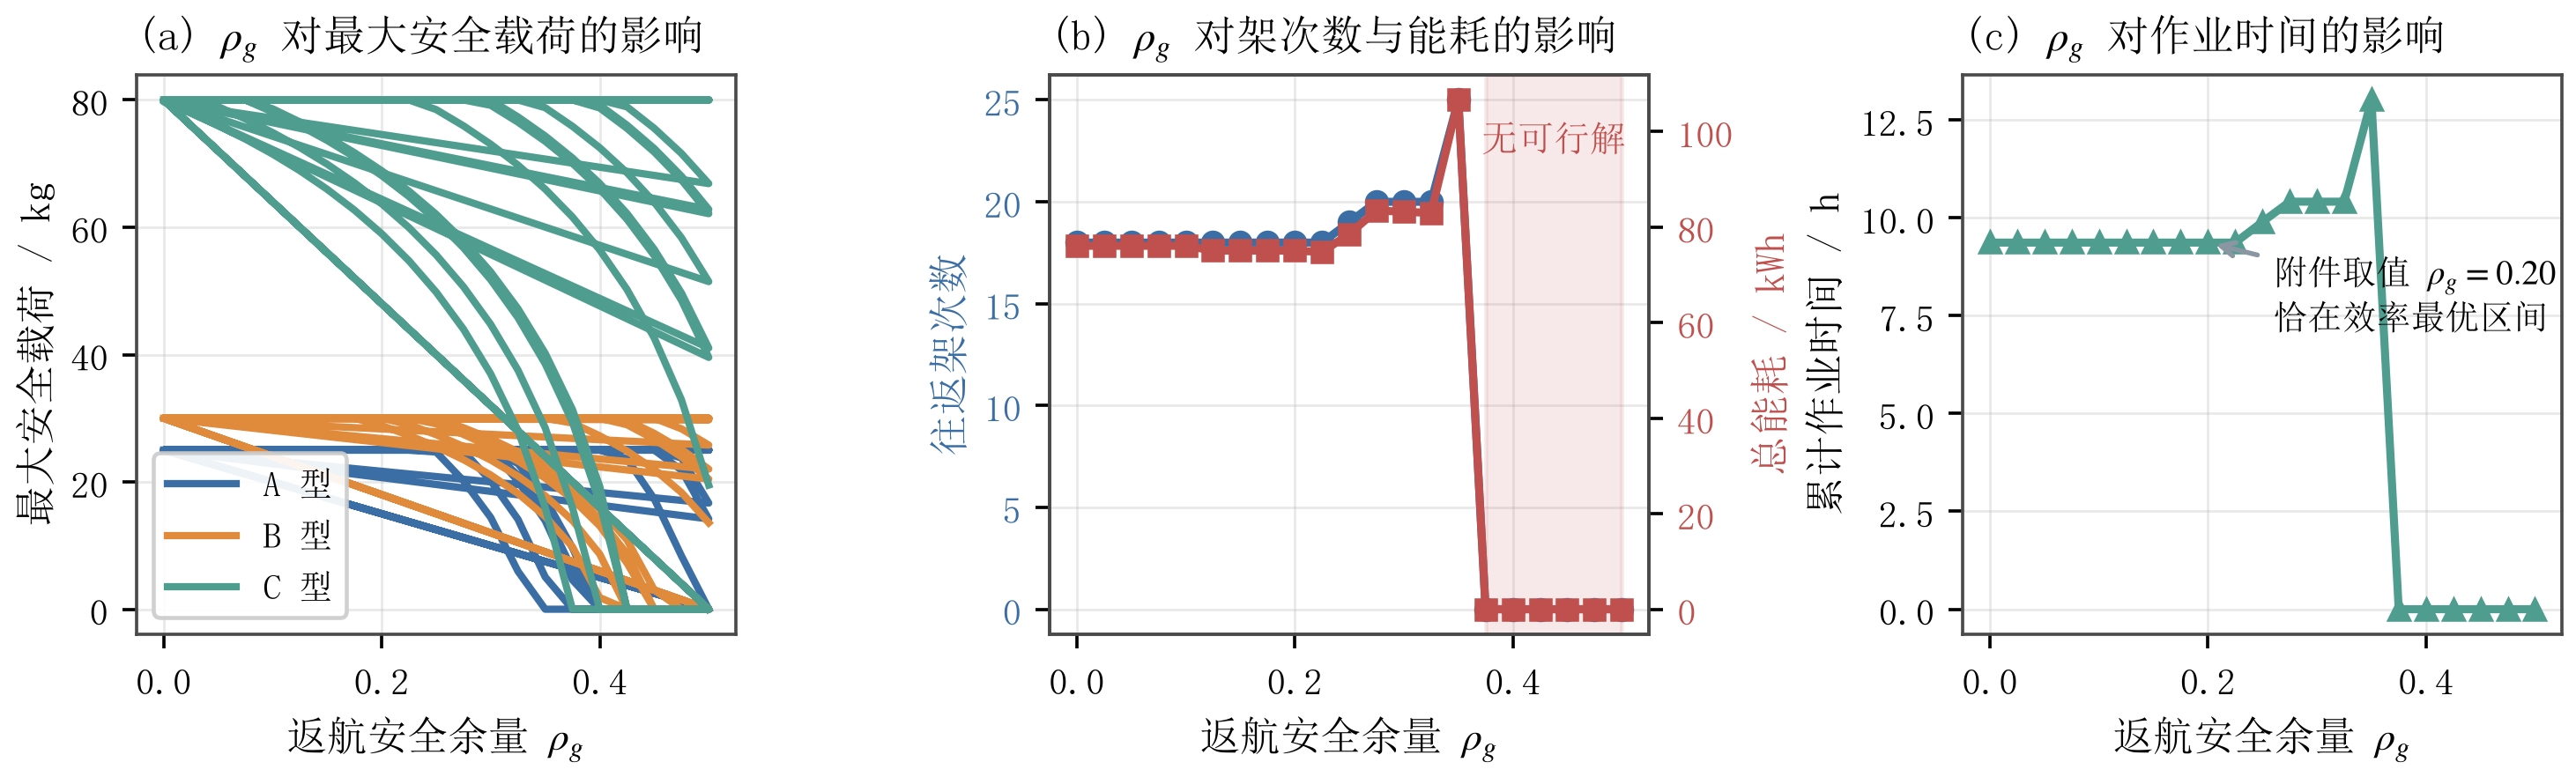
\includegraphics[width=0.98\textwidth]{figures/fig18_q1_rho.png}
	\caption{返航安全余量敏感性分析}
	\label{fig:q1_rho}
\end{figure}

由图~\ref{fig:q1_rho}(b)(c) 可得三条定量结论：\textbf{①}$\rho_{g}$ 由附件的 0.20 增至 0.35 时，架次数由 \textbf{18 增至 25}（$+38.9\%$），总能耗由 \textbf{75.07 升至 106.60\,kWh}（$+42.0\%$），累计作业时间由 9.37\,h 升至 13.01\,h；\textbf{②}在 $\rho_{g}\le0.225$ 区间架次数保持 18 不变（说明该区间内能量均非紧约束，与"结构载重主导"的结论一致）；\textbf{③}$\rho_{g}\ge0.375$ 时\textbf{问题开始无可行解}——部分远距离服务区即使空载也无法返航。

\begin{figure}[htbp]
	\centering
	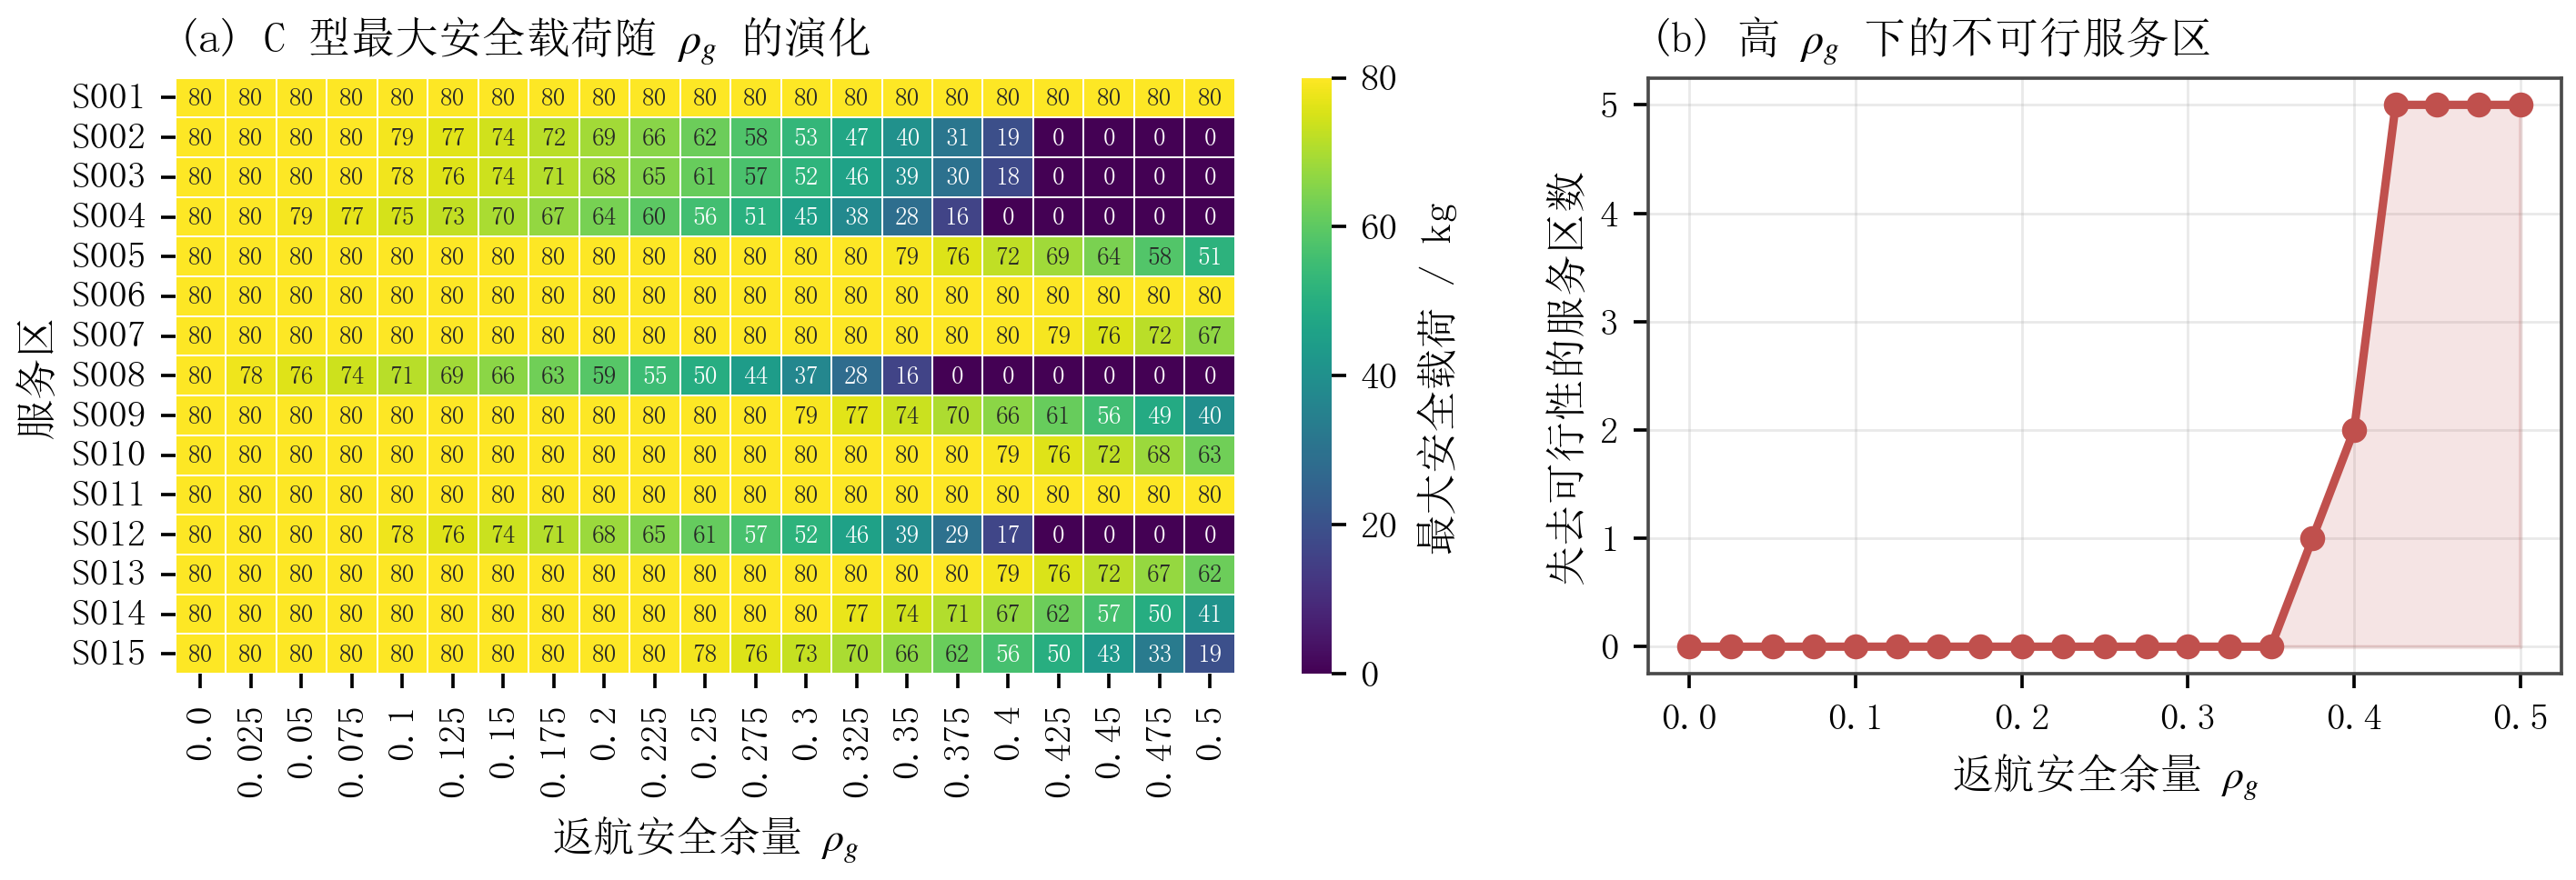
\includegraphics[width=0.98\textwidth]{figures/fig19_q1_rho_heatmap.png}
	\caption{最大安全载荷随返航安全余量的演化}
	\label{fig:q1_rho_heatmap}
\end{figure}

图~\ref{fig:q1_rho_heatmap}(a) 的热力图展示了 C 型最大安全载荷随 $\rho_{g}$ 的完整演化过程：图中颜色由深到浅对应载荷下降，远距离服务区（S008、S004、S003、S002、S012）率先变色，而近距离服务区直到 $\rho_{g}$ 很大时才受影响。图~\ref{fig:q1_rho_heatmap}(b) 给出不可行服务区数的变化：$\rho_{g}=0.375$ 时首次出现 1 个不可行服务区，$\rho_{g}=0.40$ 时增至 2 个，$\rho_{g}\ge0.425$ 时固定为 5 个（S002、S003、S004、S008、S012——正是图~\ref{fig:q1_binding}(b) 中受能量约束的 5 个服务区）。

\textbf{物理解释}：这 5 个服务区的共同特征是"距离远且沿线地形高"。以 S008 为例，单向距离 8.08\,km、航段沿线最高点 367\,m，去程爬升 96\,m；当 $\rho_{g}$ 增大到 0.325 以上时，可用能量已不足以支撑空载往返，此时\textbf{无论装载多少货物都无解}。这一结论说明附件的 $\rho_{g}=20\%$ 取值是合理的：它既保证了足够的安全裕度，又恰好处在"架次数不变"的高效区间内（$\rho_{g}\le0.225$），是安全性与效率的良好折中。
